\graphicspath{{chapters/GeneticFingImages/}}
\chapter{Genetic Figerprinting}

\textbf{\textit{Written by Elisa Bugani}}\\

Genetic fingerprinting is a tecnique used to identify some characteristics of a
genome (a pattern of variable elements), like SNPs or minisatellites, in order
to \textbf{uniquely characterize a genome}. Genetic fingerprinting can be used
to compare a genome with a reference sample or to compare different genomes
between each other, in order to determine their diversity or analogy. 

DNA fingerprinting is applied in different fields:

\begin{itemize}
	\item In \textbf{Forensic}, for identification purposes;
	\item In \textbf{lineage related tests}, for cells or humans. Eg. pternity
	test, hereditary tests.
	\item For the certification of the \textbf{origin of cells used in the
	laboratory}, to make sure that the cells are the right ones and that there
	are no major geentic drifts. Needed when using certain cell lines, for
	publishing purposes.
\end{itemize}


\textbf{Variants used for genetic testing}

There are different variants that can be used for genetic fingerprinting, such
as Single Nucleotide Polimorfisms (SNPs) or inherited Copy Number Variations
(CNVs) (see chapter \ref{chap: Basics}). Basically everything that is inherited
and that is a polimorphism can be used in genetic testing, however some variants
are more amanable than others. 

SNPs are the most amenable ones since they are simple, abundant in the genome
and easy to detect in sequencing data at any coverage depth. For these reasons,
in this lesson we will focus on the development of \textbf{SNP-based genetic
tests}.

\section{SNPs features}

\subsection{Hardy-Weinberg equilibrium and Minor Allele frequency}

One property of SNPs which has to be taken into account when using SNPs for
genetic testing is the \textbf{Hardy-Weinberg equilibrium}. In population
genetics, the Hardy-Weinberg equilibrium states that allele and genotype
frequencies in a population will remain constant from generation to generation
under neutral selection, so in the absence of other evolutionary influences,
like genetic drift, mate choice, sexual selection, mutations, population
structures. Also, it requires randomness in sexual matings, equal proportions of
males and females, infinite size.

In the simple cases following the Hardy-Weinberg equilibrium, a single locus
with two alleles denoted \emph{A} and \emph{a} with frequencies $f(A) = p$ and
$f(a) = q$, respectively, the expected genotype frequencies under random mating
are $f(AA) = p^{2}$ for the AA homozygotes, $f(aa) = q^{2}$ for the aa
homozygotes, and $f(Aa) = 2pq$ for the heterozygotes. In the absence of
selection, allele frequencies $p$ and $q$ are constant between generations, so
equilibrium is reached. 

SNPs that respect this equilibrium are also the most studied, thus more
informative. 
% #why this? #TODO

\subsection{Minor Allele Frequency}

Also, when performing genetic fingerprinting, the aim is to maximize the
probability to have different genotypes in unrelated individuals. For this
reason, the more advantageous SNPs will be the ones in which the allelic
frequency of the variants is the higher possible. Highest variability in the
population allows to distinguish better more individuals. 

Number-wise, a frequency of $\frac{1}{3}$ for each SNP would maximize the
variability, but those SNPs wouldn't be in HW equilibrium and we might have
missed calls. Therefore, the optimal SNPs to detect individuals’ differences and
similarities are those with genotype frequencies: $P_{AA} = 0.25$, $P_{BB} =
0.25$, $P_{AB} = 0.5$. $50\%$ of individuals for that SNP will have a
heterozygus genotype, $25\%$ a homozygus genotype for the reference allele,
$25\%$ for the alternative allel.

This is equivalent to say that best SNPs will be the ones with \textbf{MAF} =
0.5. Minor allele frequency (MAF) is the frequency at which the second most
common allele occurs in a given population.

% why this? #TODO

\bigskip
Some useful projects:
\begin{itemize}
	\item \textbf{dbSNPs}: is a database of small scale nucleotide variants. The
	database includes both common and rare singlebase nucleotide variation
	(SNV), short (=< 50bp) deletion/insertion polymorphisms, and other classes
	of small genetic variations. \url{https://www.ncbi.nlm.nih.gov/snp/}.
	
	\item \textbf{HapMap3}: is the third phase of the HapMap project whose aim
	is to develop a haplotype map of the human genome to describe the common
	patterns of human genetic variation in order to allows researchers to find
	genes and genetic variations that affect health, disease and individual
	responses to medications and environmental factors. The HapMap is a catalog
	of common genetic variants that occur in human beings. It describes what
	these variants are, where they occur in our DNA, and how they are
	distributed among people within populations and among populations in
	different parts of the world.
	\url{https://www.sanger.ac.uk/resources/downloads/human/hapmap3.html}
\end{itemize}

\subsection{Haplotype Blocks}

Another important feature to consider for SNPs selection are \textbf{Haplotype
blocks}. Haplotype blocks are blocks along the genome that tend to be inherited
as segments. In these sizable regions there is little evidence for historical
recombination and only a few common haplotypes are observed. 

So for example, if there are 10 SNPs in a block of 1 MB, the genotype of one
specific SNP in that block gives an indication the genotype of the other SNPs in
the same block, since they are inherited together. Hence, if there is a
haplotype block, there is no point in sequencing all SNPs in that block, it is
sufficient to select some specific SNPs. Also, when running a fingerprint assay,
there is no point in using all SNPs in a haplotype block since they won't bring
additional information independently.

SNPs in the same HB are said to be in \textbf{Linkage Disequilibrium} (LD).
Linkage disequilibrium measures the non-random associations between alleles or
polymorphisms at different loci. A higher LD indicates a SNPs with a stronger
tendency to co-segragate. Haplotype Blocks are therefore commonly represented
with \emph{linkage disequilibrium plots} \ref{fig:LD_plot}. In these plots, SNPs
are represented in a way that does not respect the genomic distance, but the
order along the genome (position of each SNP relative the others). \\

\begin{figure}[ht]
	\centering
	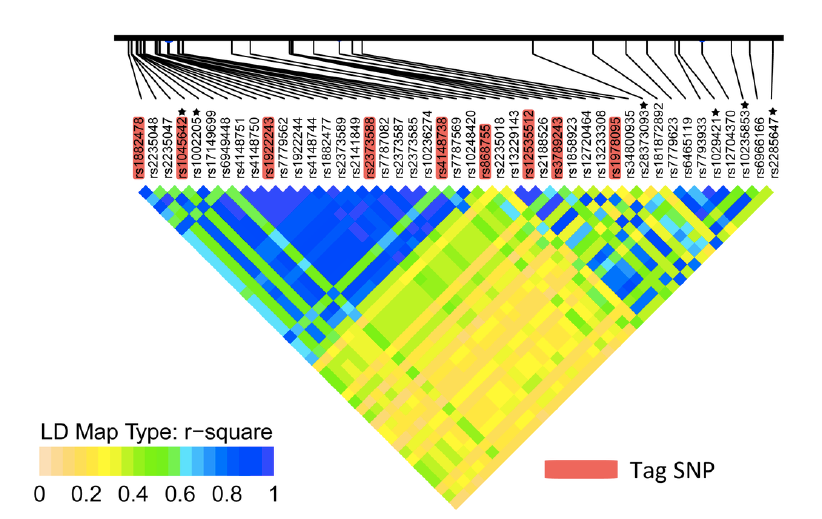
\includegraphics[width=0.95\textwidth]{LD_plot.PNG}
	\caption{Linkage disequilibrium plot.} 
	% #TODO come andrebbe letta esattamente?
	\label{fig:LD_plot}
\end{figure}


In figure \ref{fig:LD_plot}, the colors indicate the strenght of pairwise
linkage disequilibrium (LD) according to r2 metrics. Tag SNPs are shadowed in
pink. A \textbf{Tag SNP} is representative of a region with high linkage
disequilibrium and represents a group of SNPs (called haplotype).


\subsection{Other SNPs features} 
\begin{itemize}
	\item Choose SNPs that are in areas that are not likely to undergo somatic
	aberrations. So \underline{exclude chromosomal locations which undergo
	frequent somatic aberrations}. Eg. areas commonly deleted in tumor will
	produce LOH but probably also no calls, since there is no DNA. 
	\item Choose \underline{SNPs equally represented}/spread all around the
	genome (not in specific chromosome regions).
	\item Select \underline{autosomal only SNPs}.
	\item Select \underline{SNPs in exons}. If we were to run a targeted assay,
	this would cover more exons instead of intrones. It will also be more
	probable to have signal from a non-DNA assay, for example if calling a
	genotype from RNA sequencing data (even though it is not always done).
	\item Exclude/include \underline{disease or drug response associated loci}. 
	\item Include/exclude loci with significantly \underline{different MAF in
	different ethnicity}. If we include them we can also have a lineage type of
	tests in the same assay. 
\end{itemize}


\subsection{Number of SNPs to select} 

If we want to build a test to run genetic fingerprinting using SNPs, \textbf{how
many polymorphic loci (SNPs) should be tested?} We want to make sure that the
measure of the test will be able to differentiate unrelated individuals. But we
must also remember that many variables must be taken into account, possible
mismatches in particular. Those can be due to the sequencing process itself
(experimental mismatches) but also to changes due to somatic events (biological
mismatches). All these events can be used in the test with a different weight,
based on how likely they are. 


\subsubsection{Experimental mismatches : Genotype call error rate}

During sequencing, each machine will produce some errors, resulting in some loci
for which no data will be available. If those loci include some SNPs of
interest, then no call will be associated to that SNP. Experimental mismatches
are related to the error rate of the technology used, they are platform
dependent. 

\paragraph{Some examples:}

\begin{figure}[ht]
	\centering
	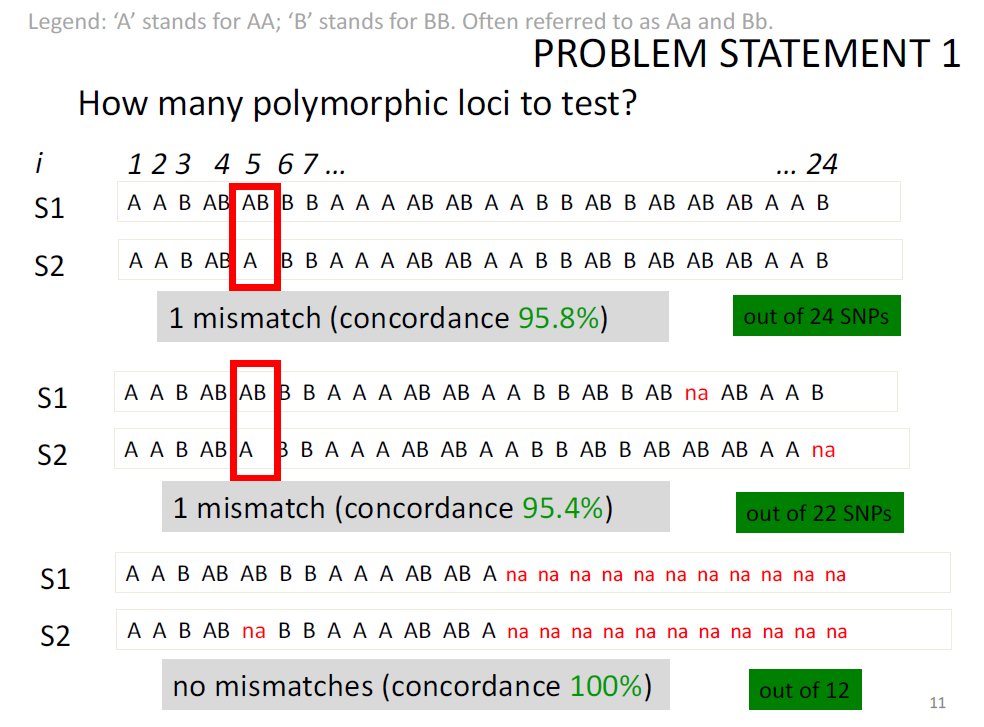
\includegraphics[width=0.7\textwidth]{SNP_number.PNG}
	\caption{'A' stands for 'AA' (e.g. homozygus genotype for the reference
	allele); often refered to as Aa. 'B' stands for 'BB' (e.g. homozygus
	genotype for the alternative allele); often refered to as Bb. 'AB' stads for
	heterozygus.}
	\label{fig:SNP_number}  
\end{figure}

In each example in figure \ref{fig:SNP_number} there are two samples with the
same number of potential SNPs: 24. To detemine the difference/similarity
(concordance) of the two samples we can look at the genotype for each position
and count mismatches.

Legend: 'A' stands for 'AA' (e.g. homozygus genotype for the reference allele);
often refered to as Aa. 'B' stands for 'BB' (e.g. homozygus genotype for the
alternative allele); often refered to as Bb. 'AB' stads for heterozygus.

\begin{itemize}
	\item \textbf{First Example}: over the 24 loci, there is only one mismatch.
	This translates to a level of concordance of 95.8\%. Those 2 individuals are
	highly related or DNA comes from the same saples. 
	   
	\item \textbf{Second example}: there is only one mismatch but there are some
	'na', indicating that for some positions we don't have a call (not available
	data). Therefore, in this case the concordance is measured out of 22 SNPs
	and is equal 95.4\%. 

	\item \textbf{Third example}: here a lot of 'na's are present, leading to
	have only 12 SNPs available. This brings to a concordance of 100\%. 
\end{itemize}

Different examples produced different levels of concordance. What do we trust
the most?

The first set of SNPs is the one that we trust the most, because it has the
higher number of available SNPs. Wider number of SNPs provides the most reliable
information. 

\subsubsection{Biological mismatches}

In the context of desease samples and tumors, many somatic events can happen,
like deletions, gains of copies, homozygus deletions, ecc. Some common ones are:
\begin{itemize}
	\item  \textbf{Loss Of Heterolzygosity (LOH)}:  event that results in loss
	one parental copy of a region which results in the genome having just one
	copy of that region. If that region contained a heterozygus locus (e.g.
	SNP), there will be loss of Heterozygosity. $AB \rightarrow A$.
	\item \textbf{Gain Of Heterozygosity (GOH)}: due to a mutation in a site
	often polimorphic through inheritance. These are pretty rare. $A \rightarrow
	AB$. 
	\item \textbf{Double Mutation (DM)}: very rare.  
\end{itemize}

\begin{figure}[ht]
	\centering
	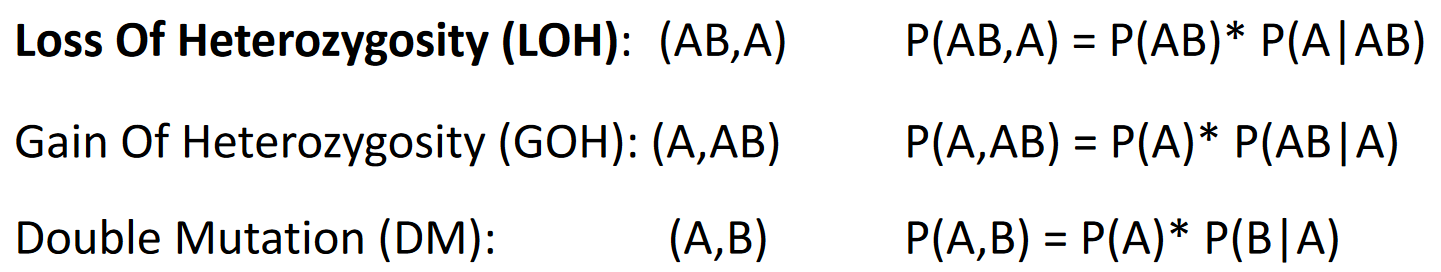
\includegraphics[width=0.75\textwidth]{heterozygosity.PNG}
	\caption{} 
	\label{fig: heterozygosity}
\end{figure}

\bigskip
Biological mismatches can be properly modeled in our assay. We can, in a data
driven way, assess the error rate for the genotyping for some specific SNPs or
run tests. We can also think in terms of SNP-specific or tissue-specific
probabilities.

The main point is that all mismatches must be taken into consideration. For
this, all implemented tests use \emph{more than the minimal number of SNPs} that
allow to identify individuals. 


\section{Genetic Distance}

Having defined the number of SNPs to use, with maximum MAF and other amanable
characteristics, the genetic test should provide a measure of some sort, which
will be the output metric, associated with a probability of the measure to be
correct. \\

As a simple measure, we can \underline{count the number of loci where two
samples show different genotype} and normalize on the total number of queried
loci, defining a certain level of discordance (or concordance). The output value
will be the '\textit{genetic distance}' between the two samples given the
selected loci. The distance is proportional to the number of discordant calls.
\\

In figure \ref{fig:Distance} we can see an example of a typical graph used to
measure the genetic distance using SNP-based genetic testing. We have 4 samples
with a set of 5 SNPs for each one. The distance is measured among all possible
pairs, whose indexes are reported on the x-axis. 

\begin{itemize}
	\item s1 and s2 have 3 A in common, one locus has no call and another one
	produces a mismatch. 1 mismatch out of 4 produce a distance of 0.25.
	\item samples s1 and s3 have 5 mismatches out of 5, so a distance (or
	discordance) of 1. 
\end{itemize}


\begin{figure}[ht]
	\centering
	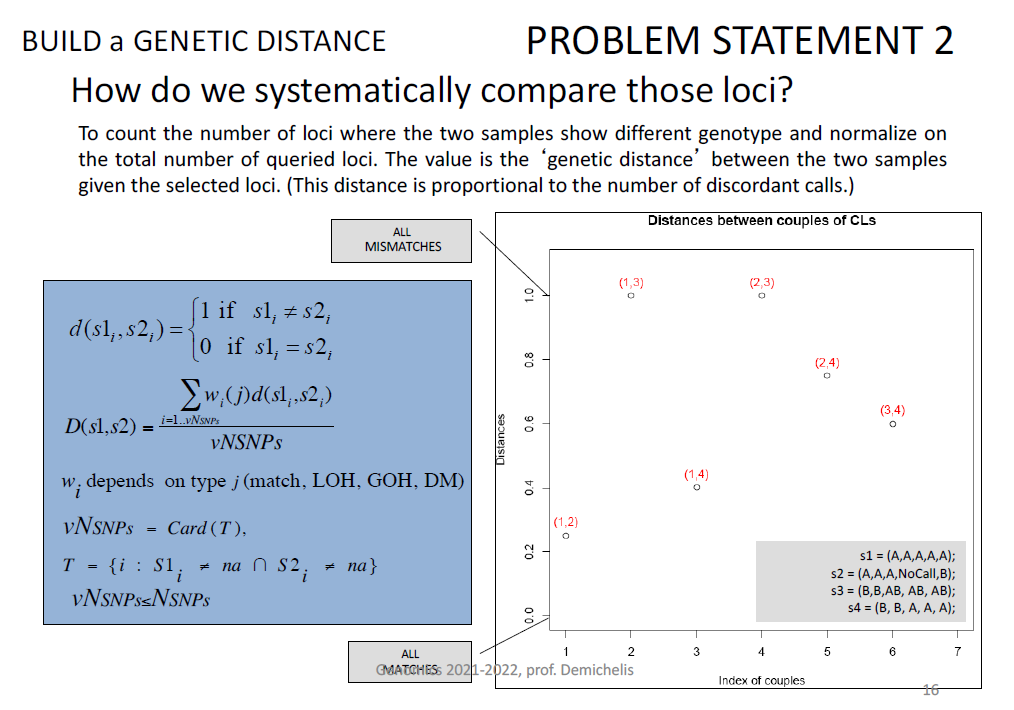
\includegraphics[width=1\textwidth]{Distance.PNG}
	\caption{Genetic Distance graph with 4 samples}
	\label{fig:Distance} %#TODO metti label sotto caption
\end{figure}

If we put that into an equation in \ref{fig:Distance} will have that: for each
position $i$ (SNP) bwteeen sample 1 and 2 we can have 1 if the genotype is
different, 0 if they are identical. Then we determine the distance D by summing
up the different scores obtained for each SNP. We can associate different
weights $w_i$ to different mismatches (depending on Gain Of Heterolzygosity,
Loss Of Heterolzygosity, Double Mutation) or we can put all equal to one. Then
we devide by the total number of SNPs for which we have available calls vNSNPs
for both the sequences in comparison, which will be lower or equal to the total
number of SNPs, NSNPs. 


\begin{figure}[ht]
	\centering
	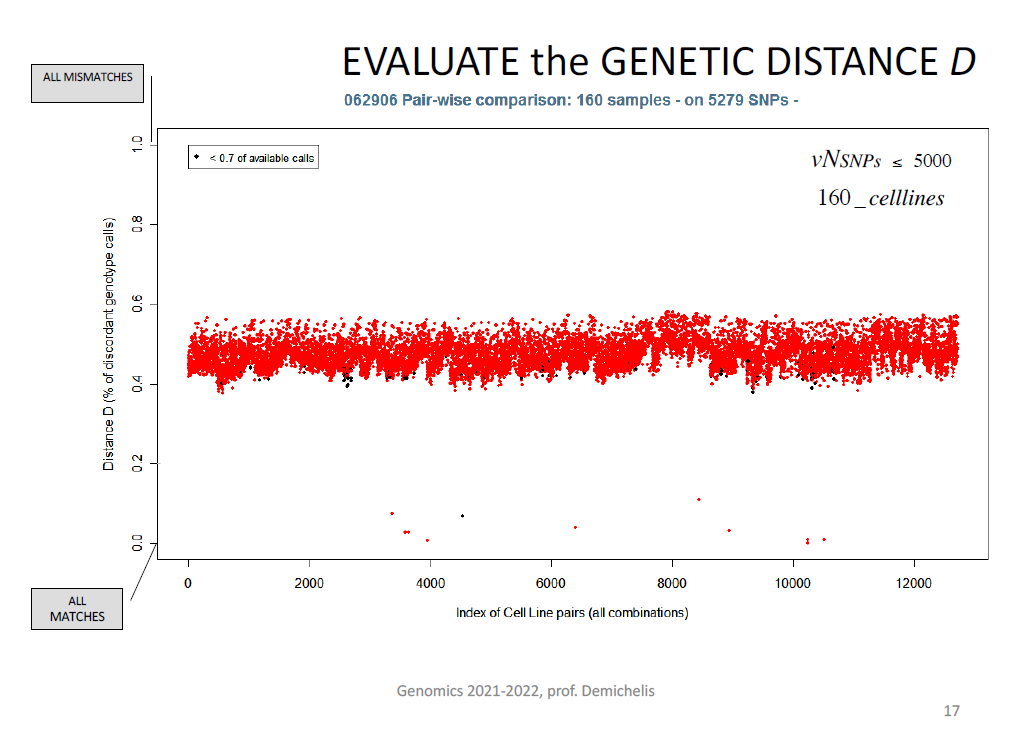
\includegraphics[width=0.9\textwidth]{Distance2.PNG}
	\caption{\label{fig:Distance2}Genetic Distance graph with 160 samples}
\end{figure}

\bigskip
This other example at figure \ref{fig:Distance2} shows the distance, measured by
genetic fingerprinting, of a collection of 160 samples of cell lines. 

The number of possible pairs corresponds to: $\frac{160 \cdot 159}{2}$ (number
found in the x-axis). 

By applying this measure to a larger collection of samples like this one, with
many SNPs, we expect to find an \textbf{average distance} among all possible
pairs that very unlikely will be close to 1. 

The MAF of the SNPs is 0.5 but it will never happen that, with a high number of
SNPs, the discordance will be 1, meaning that the SNPs will be all different. We
will have an average distance that in this case around 0.5, since by chance we
all share some genotypes on a large number of SNPs. 

Here they found certain pairs with a very low distance, sometimes almost equal
to zero (dots at the bottom). This was a surprising result because it shows that
those pairs, which were suppose to be different cell lines, were actually not
different cell lines (only less than 70\% of SNPs have available calls). 


\begin{figure}[ht]
	\centering
	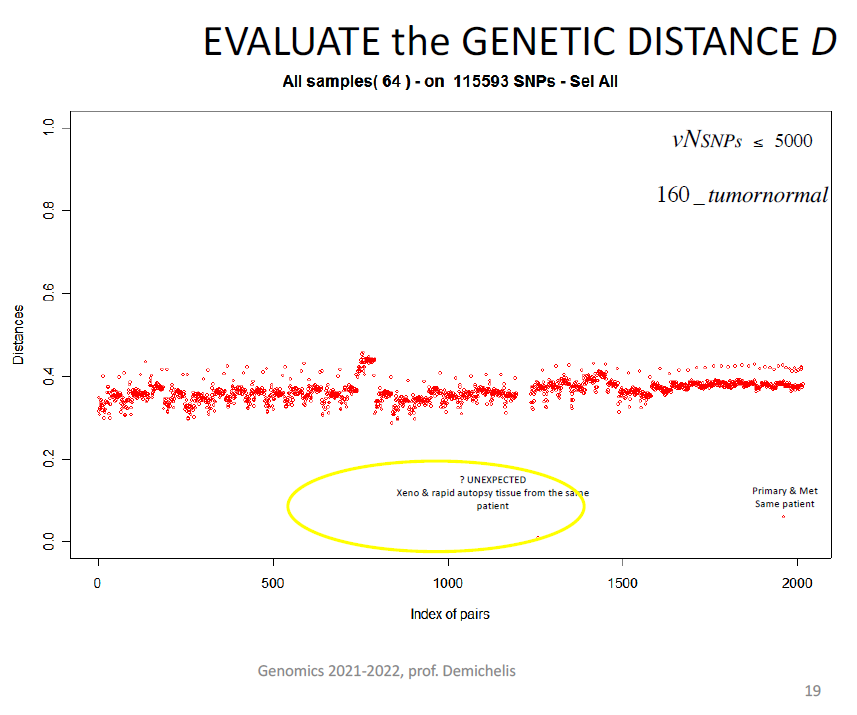
\includegraphics[width=0.9\textwidth]{Distance3.PNG}
	\caption{\label{fig:Distance3}Genetic Distance graph with tumor samples}
\end{figure}

\bigskip
In this last example at figure \ref{fig:Distance3} genetic fingerprint was
performed on a collection of 160  tumor samples, with a larger SNP array (more
that 100.000 SNPs).  

From the analysis, two samples with very low distance were observed. One of the
two samples came from a Rapid Autopsy Progam and the other one from a xenograft
model. 

\underline{RAP} are programs for which patients at the end of their life agree
to donate their tumor tissues which can be used for research. In these very
complex but highly valuable programs, the material must be taken within two
hours after death. Those samples are usually higly caractherized but after a
while the track of the patient's identity is lost. Here, what happened is that
one man who donated tissue to this program was sequenced and for some of those
metastasis models were generated and implanted into a mouse and a xenograft
model was derived. Thanks to fingerprinting it was possible to determine the
same origin between xenograft and patient. 

The power of this tecnique is very high, it allows also to identify and remove
things that we don't want in our study. Eg. if running a study (like a GWAS
study) on a certain \underline{interesting geopraphic area}, we will want to
remove the members of the same family because that would skew the results.
Genetic fingerprint can be used for this purpose.

\subsection{Some questions}

\noindent\textbf{Q1}: \textbf{\textit{Would the average of unrelated samples
distance increase or decrease after selection of ideal SNPs?}}\\

If we use SNPs likely to be different among individuals and we use them to
determine the measure of the ditance, then the average value of unrelated
individuals will increase.\\

\noindent\textbf{Q2}: \textbf{\textit{Is it likely to obtain a genotype distance
D = 1?}}\\

We get distance 1 only if we are looking at too few viable SNPs. Whereas with a
well selected pool of SNPs, and a high enough number of SNPs, it is very
unlikely that the distance is equal to 1.

\subsection{Further considerations}
How does the genetic distance among different samples change when varying the
number of selected SNPs used to perform the test?

\begin{figure}[ht]
	\centering
	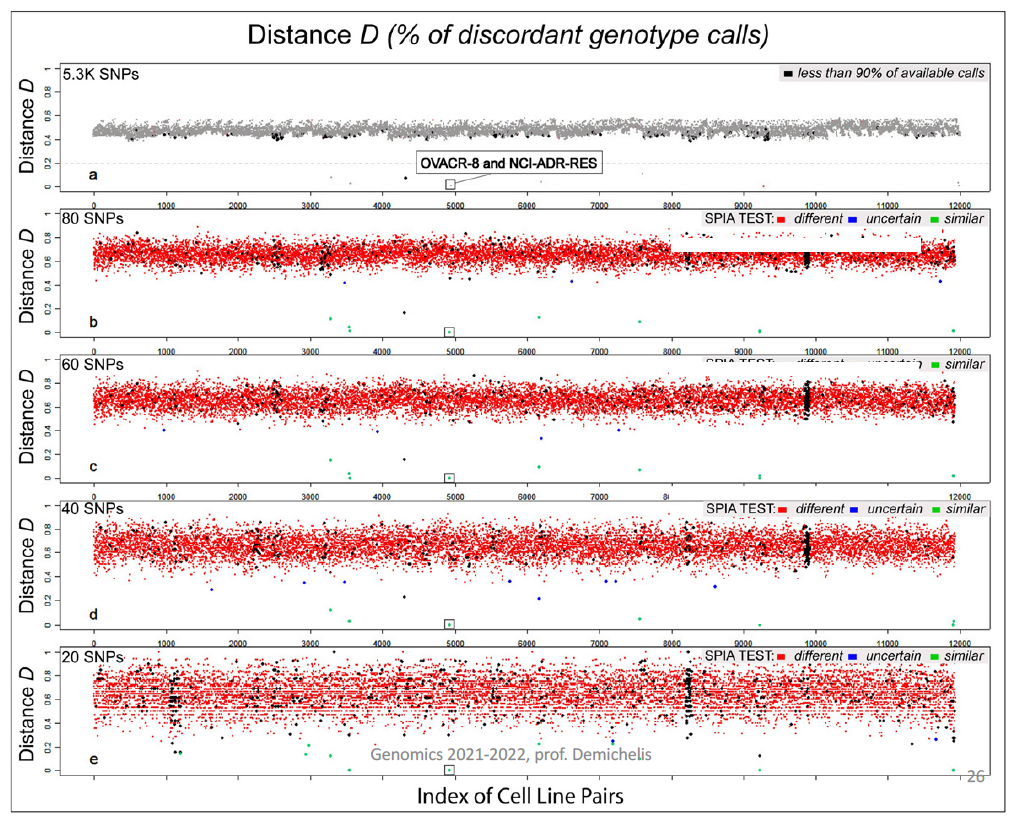
\includegraphics[width=1\textwidth]{Selected_SNP.PNG}
	\caption{Genetic Distance graph at deacreasing number of selected SNPs}
	\label{fig:sel_snp}
\end{figure}

The genetic distance among many samples, with an array of 5.3K SNPs, was
measured, using a decreasing number of SNPs (from the initial total number of
SNPs to decreasing numbers of highly selected SNPs) \ref{fig:sel_snp}. \\

It is noticeable that, in the second plot where 80 SNPs matching the required
characteristics were selected, the average Distance across all pairs is higher
than in the previous example, in which all available SNPs were used ($\sim 0.45$
vs. $\sim 0.65$). Also, the standard deviation of greater. Decreasing the number
of SNPs to 60, then to 40 and 20 leads to have the same average distance between
pairs, which settles around 0.66, but higher standard deviation.

In reality we always need enough SNPs, enough information, in order to prevent
unexpected issues and to be sure that for any pairs of sample we have enough
information to trust our measure. 


\section{Building a SNP-based genetic test}

Building an identity test base on SNPs is a MULTI-STEP process, consisting in: 
\begin{enumerate}
	\item Definition of a genotype/genetic distance to compare samples;
	\item Definition of SNPs requirments, based on the intention of the assay.
	\item Selection of SNPs:
	\begin{itemize}
		\item This can be done in a data-driven manner, through an iterative
		procedure of training and test on known sample set;
		\item Or, performing the selection based upon MAF and Hardy-Weinberg
		equilibrium. For example, using HapMap data.
	\end{itemize}
	\item Implementation of a probabilistic test (different, uncertain or
	similar)
	\item In silico validation on independent/multiple dataset.
	\item Validation on cell lines genotyped on independent platform. 
\end{enumerate}
We have already seen some of the steps needed (1, 2, 3), we now pass to the
following ones.


\subsection{Implementation of a probabilistic test} 

Other important questions which we have to answer to when designing a genetic
test are:
\begin{itemize}
	\item What is the \textit{threshold} on the genotype distance to call two
	samples 'identical' ('similar') or 'different'?
	\item How \textit{confident} would the call be?
    \item What is the \textit{minimum number} of loci needed for a robust test?
\end{itemize}

It could be useful to have a probabilistic test to determine if the measure of
the test is correct at which level of confidence. We can use a probabilistic
approach to compare observations with expectations (gold standard).

\bigskip
Under the assumption that SNP calls at different loci are independent, we can
think in terms of Binomial distribution. Each SNP can be considered as a trial,

\begin{itemize}
	\item $n$ = number of SNPs in the assay, 
	\item $k$ = number of matches, 
	\item $p$ is the probability of match and ($1-p$) of mismatch.
\end{itemize}

Then the probability of having k matches (successes) out of N SNPs (trials)
follows the binomial distribution. With $n$, $np$ and $np(1-p)$ large enough, we
can use the \textbf{Gaussian approximation} of the Binomial distribution with
$K_{\text{mean}} = np$ and $sd = \sqrt{np(1-p)}$. \\


\begin{figure}[ht]
	\centering
	\begin{subfigure}[t]{0.80\textwidth}
		\centering
		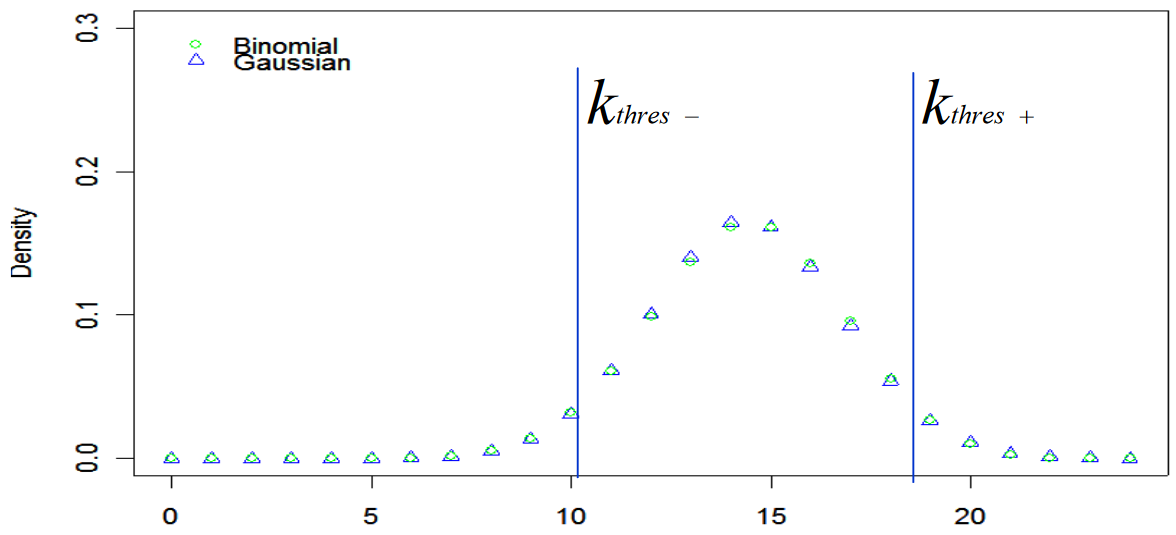
\includegraphics[width=1\textwidth]{binomialDistSNPsmatches.PNG}
		\caption{The probability binomial distribution could be approximated to a Gaussian when the number of cases is large}
		% \label{subfig: }
	\end{subfigure}
	\hfill
	\begin{subfigure}[t]{0.80\textwidth}
		\centering
		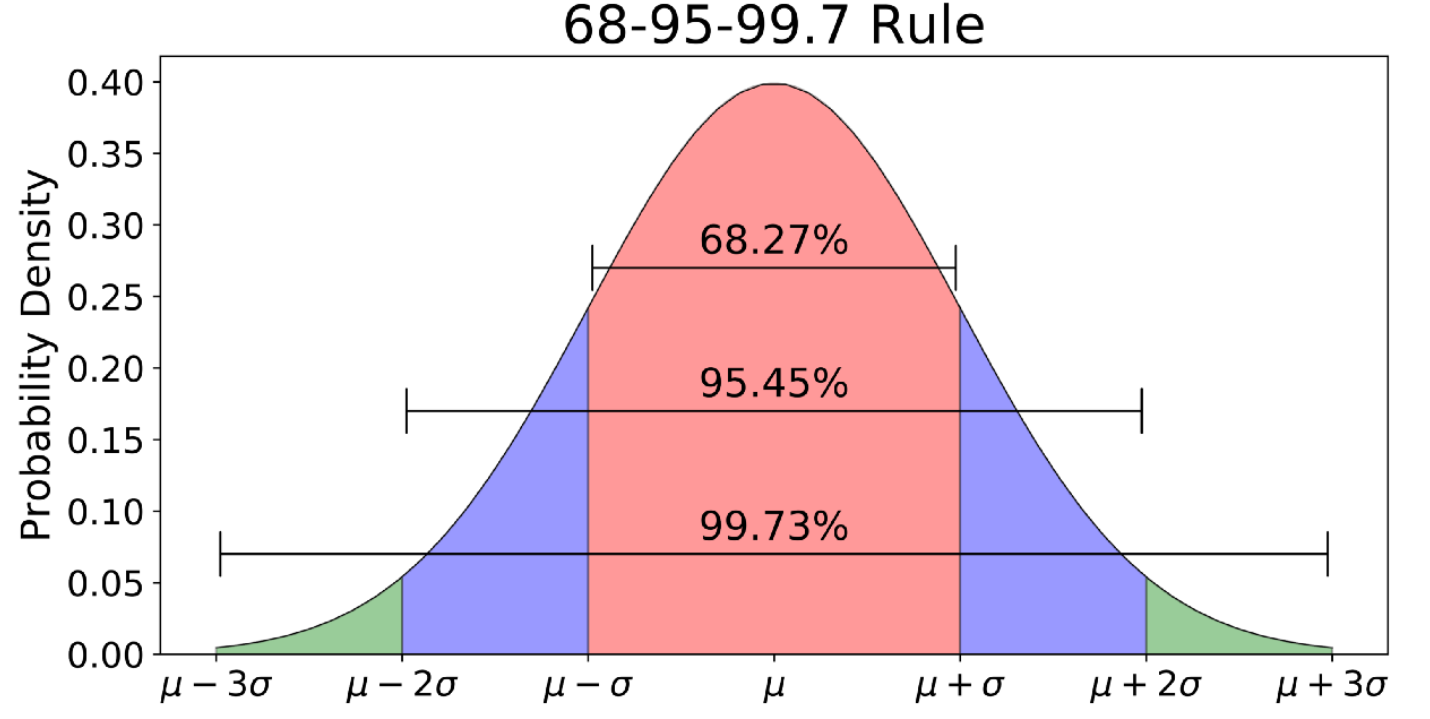
\includegraphics[width=1\textwidth]{gaussianity-binomialdist.PNG}
		\caption{Percentages Gaussian distribution}
		% \label{subfig: }
	\end{subfigure}
	\caption{Approximation of a binomial distribution to a Gaussian and
	percentages related.}
	\label{fig: binomial distribution SNP matches}
\end{figure}

With something that simple we can add a probabilistic test in our assay,
defining an area of confidence given by $K_{\text{mean}} \pm m \cdot sd$ where m
is the number of standard deviations used to define the thresholds which will
lead to have a smaller or wider confidence area. 

%immagine slide 33
\begin{figure}[ht]
	\centering
	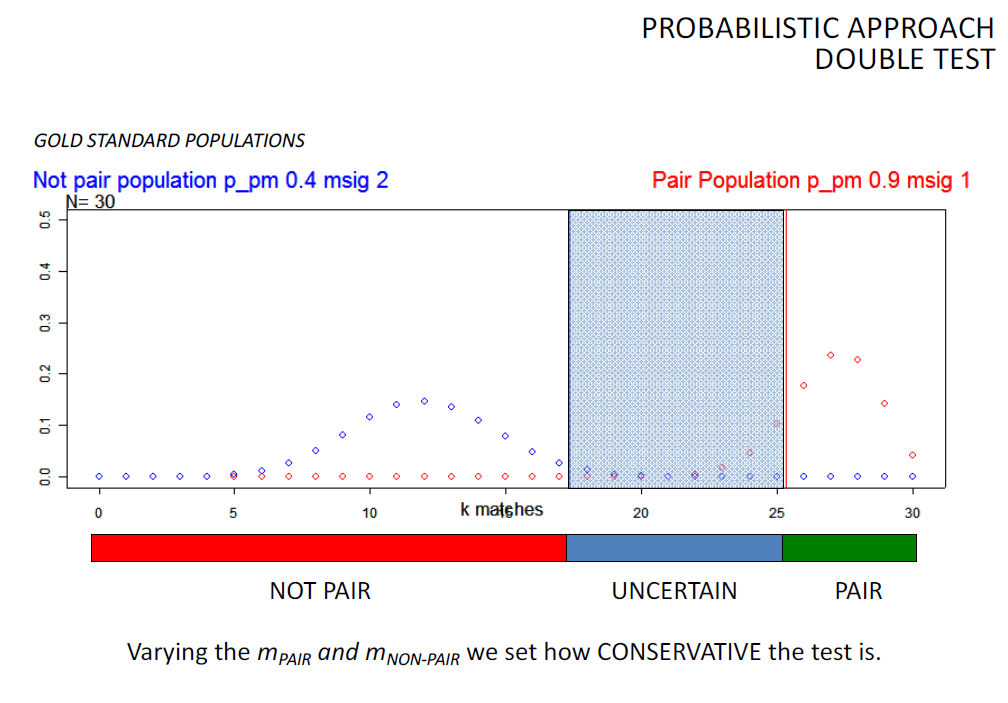
\includegraphics[width=0.9\textwidth]{Prob_test.PNG}
	\caption{\label{fig:prob_test}}
	% #TODO not pair populations? paired populations? Don't understand the
	% meaning of these things
\end{figure}


\bigskip
So for example: given two unrelated samples, we reason in terms of  
'\textit{what is the probability of having a certain number $k$ of matches over
a total number of n SNPs, therefore a certain value of D?}'.\\
\noindent The probability mass function for unrelated individuals is shown in
figure \ref{fig:prob_test} with a blue dotted line and indicates that there is a
low probability of having both a very low and a very high number of matches (it
is assumed that the comparisons of samples follow a binomial distribution, where
higher and lower values, compared to the mean, have less likely). 

\noindent We can also think in the opposite term: given two related samples,
what is the probability of having  matches? As represented by the red dotted
line, in this case there will be a high probability of having many matches. 

Using these probabilities we can set two thresholds which will define 3 regions:
\begin{itemize}
	\item A \textbf{'not pair'} region for which the two samples will be
	considered as 'different'.
 	\item a \textbf{'pair'} region for which the two samples will be considered
 	as 'similar'.
	\item and an \textbf{'uncertain'} region, a grey zone, for which no certain
	result can be produced. 
\end{itemize}

Then we can move the grey area based on what we want to be certain of and on how
many SNPs we have.

By decreasing the number of SNPs, the grey zone will become more tiny, making
the result more difficult to interpret. For example, a difference of only 2
matches could lead to opposite conclusions. 

By contrast, with more SNPs the area will be wider and easier to interpret.
Hence using a number of SNPs greater than the minimum number is better,
otherwise there will be many uncertain calls. 


\section{Further considerations and examples}
%sistemare
In the past, before sequencing area and SNPs array area, \underline{short tandem
repeats} were commonly used for genetic fingerprint. They were used on gels to
distinguish related and unrelated individuals, eg, for the initial paternity
test.\textbf{ Di-nucleotide markers} are the most informative class of
microsatellites. Generally they are more informative than SNPs, though selected
SNPs perform quite well.\\

\textbf{Inherited copy number variants} can be used too for a fingerprinting
test, but not all of them. The more amenable for this test are the loss type of
CNV. In the population there will either a copy number of 2 or 1 or 0. If both
parents have heterozygus pair of CNVs it will be possible that I have a
homozygus deletion. If both parents have 2 copies at a site that is polimorphic
in the population, we will have a genotype equal to 2 copies. \\

If we think about \textbf{gain} of CNV then it becomes messy, because when
combining multiple copies and have a add up we cannot distinguish what comes
from what pair, so we cannot use them to identify an individual.


\subsection{Example 1: Cell line passages}

A mass use of these genetic tests is done to assess \textbf{genetic changes in
in-vitro cultivation}. Cell lines go through multiple passages in which they are
used and stored. Genetic fingerprinting can be used to assess if among different
passages the cells have remained the same, if they were mislabeled or if major
genetic drifts happened. Genetic fingerptinting is also used in studies of tumor
evolution, lineage plasticity, etherogenity across metastasis across individuals
or a single tumor. 

% #TODO add to definitions
\textit{Lineage plasticity}, the ability of cells to transition from one
committed developmental pathway to another, has been proposed as a source of
intratumoural heterogeneity and of tumour adaptation to an adverse tumour
microenvironment including exposure to targeted anticancer treatments.

In this example (figure \ref{fig: cell lines comparison}), two types of prostate cell lines
which underwent multiple passagges were used: \textit{\textbf{N15C6}} (passages
from 48 to 63) and \textit{\textbf{N33B2}} (passages from 21 to 39). The cell
lines were profiled with a SNPs array and the assay was run. All passages of
each cell lines were compared with all other passages. We expect all passages to
have the same genetic fingerprinting in the same cell line.\\ 

However the results obtained using the \textbf{full array of SNPs (50k)}
(subfigure \ref{subfig: 50k SNPs}), showed that some pairs which should be
exactly identical (distance equal to zero) are actually a bit different 
% #TODO shouldn't it be correct?
(points at the bottom-left). By contrast, by using a set on only 54 SNPs
(subfigure \ref{subfig: 54 SNPs}), this diversity is not detectable, indicating
that using the restricted number of SNPs could make us loose some information. 

% #TODO ???
\begin{figure}[ht]
	\centering
	\begin{subfigure}[t]{0.80\textwidth}
		\centering
		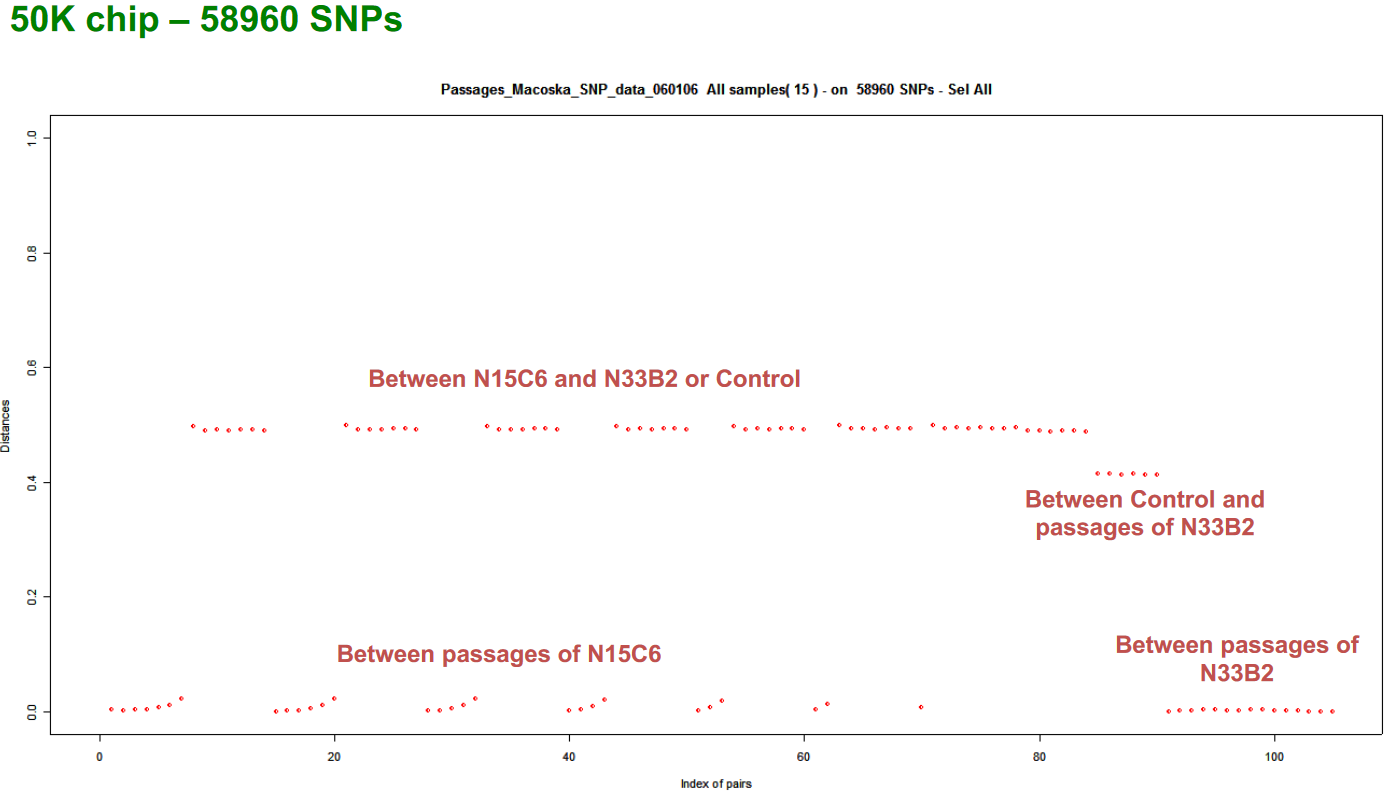
\includegraphics[width=1\textwidth]{50Kchip.PNG}
		\caption{Comparing passages with the total amount of available SNPs}
		\label{subfig: 50k SNPs}
	\end{subfigure}
	\hfill
	\begin{subfigure}[t]{0.80\textwidth}
		\centering
		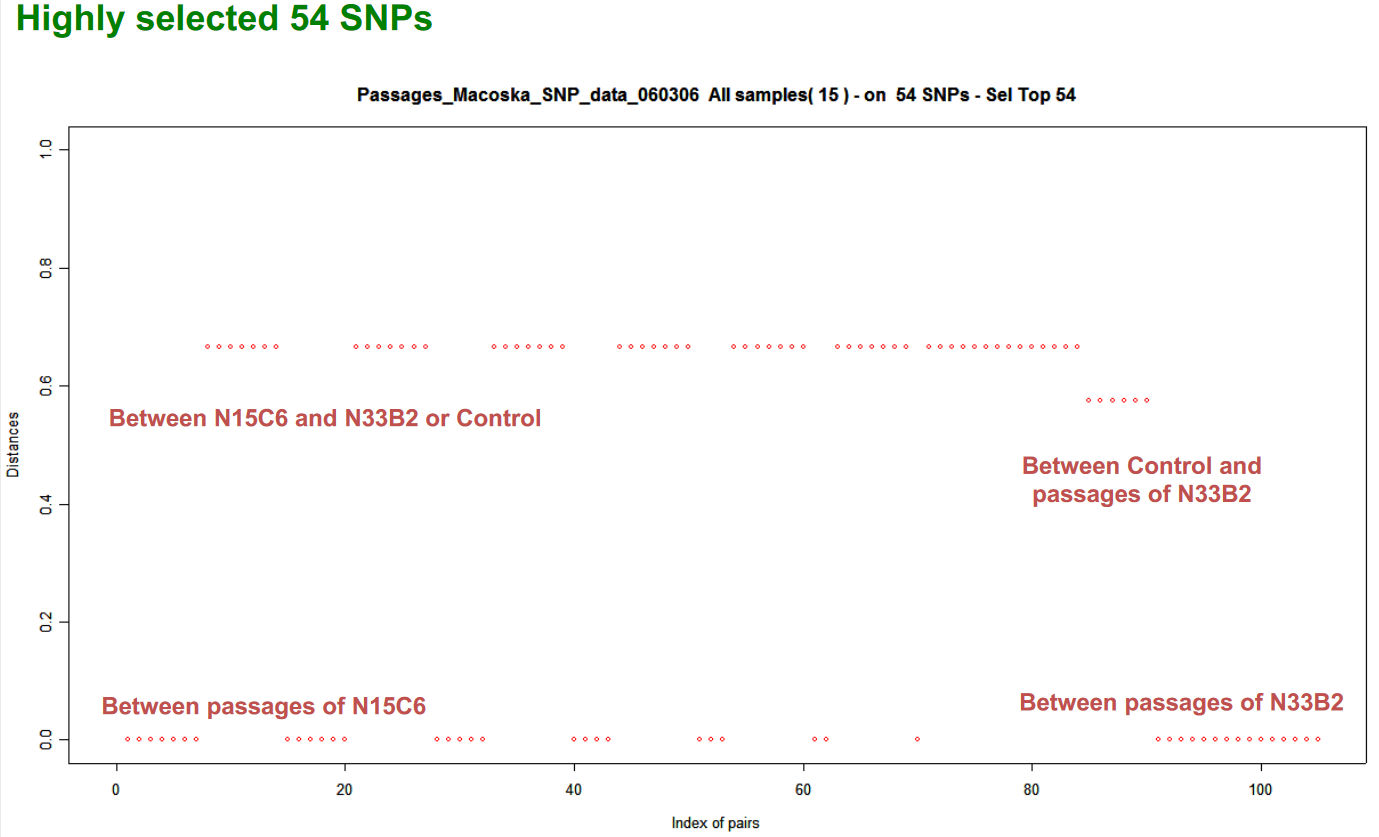
\includegraphics[width=1\textwidth]{54SNPchip.PNG}
		\caption{Comparing passages with 54 SNPs}
		\label{subfig: 54 SNPs}
	\end{subfigure}
	\caption{}
	\label{fig: cell lines comparison}
\end{figure}


In order to understand this increase of distance, they looked at each chromosome
to see if there were problems that justified increase the increased distance
expected to be equal to zero in that cell line. All chromosome were tried. If we
focus only on the SNPs spread across Chromosome 11, we observe that there is a
major difference for certain passages with respect to the initial ones, only for
one cell line (N15C6). This was due to the way the cells were immortalized
(insertion in chromosome 11), look to figure \ref{fig: chr 11 SNPs}.

\begin{figure}[ht]
	\caption{Comparison passages regarding chr 11}
	\centering
	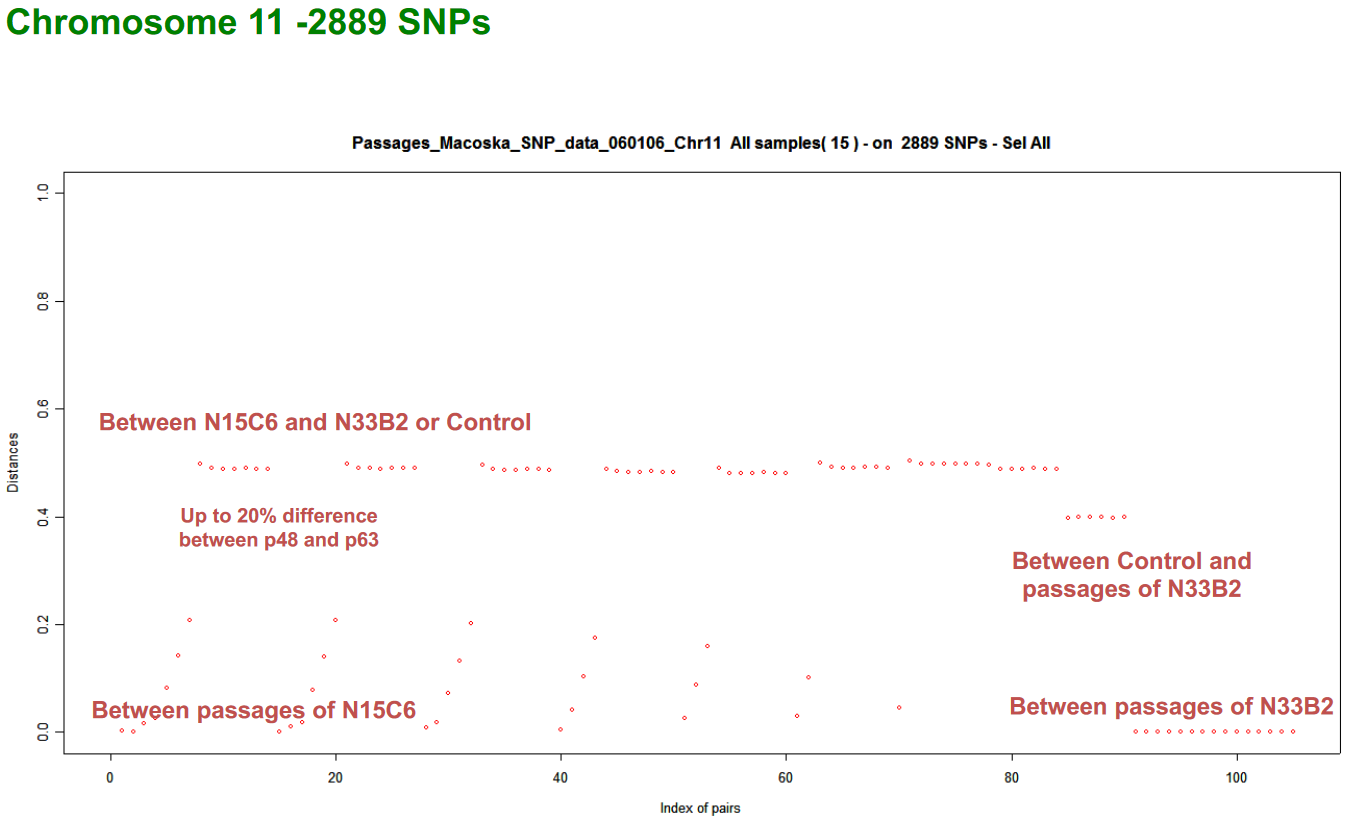
\includegraphics[width=0.8\textwidth]{chr11chip.PNG}
	\label{fig: chr 11 SNPs}
  \end{figure}


\subsection{Individual's Relatedness (genotype-distance)}

The HapMap consortium sequenced hundreds of individuals for different
ethnicities and also used trios. \textbf{Trio sequencing} is a technique which
involves the sequencing of the genome of \underline{mother, father and
son/daughter}. Trios provide major information for haplotype blocks, for
identifying regions related to inheritance, ecc.

% immagine slide 43
\begin{figure}[ht]
	\centering
	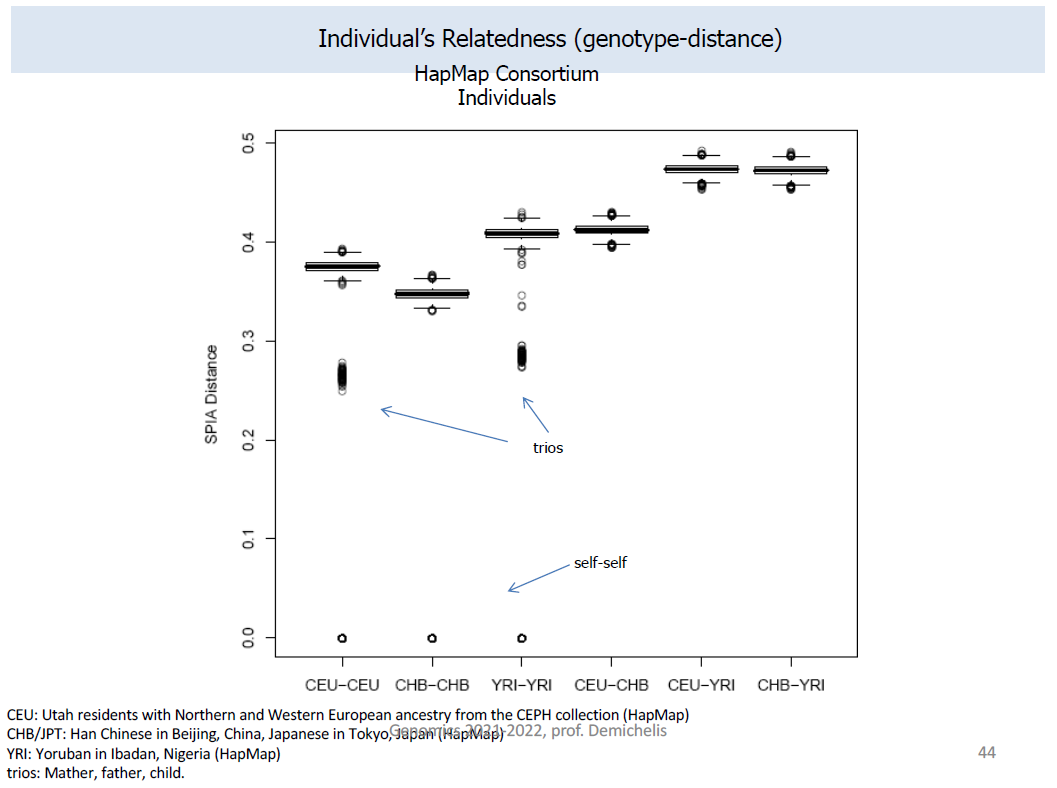
\includegraphics[width = 1\textwidth]{trios.PNG}
	\caption{\label{fig: trios}}
\end{figure}

By looking at the data based on \textit{SPIA Assay} (subsection \ref{subsect:
SPIA}) (a genotype base assay which measures distance) at figure \ref{fig:
trios} we see that self-self pairs have distance zero, as expected; samples
within each ethnicity have a certain average distance, which is lower than the
distance observed among different ethnicities. Differences in distance among
mixed samples are due to the fact that the SNPs used had on average higher MAF
in some populations than in others. \\
\noindent We also notice that in trios the distance is not 0 and is not equal to
the median distance of unrelated individuals. This can be used for paternity
tests or even in forensic science (figure \ref*{fig: Relatedness of
individuals}).

\begin{figure}[ht]
  \caption{Relatedness between individuals can be evaluated through SNPs}
  \centering
  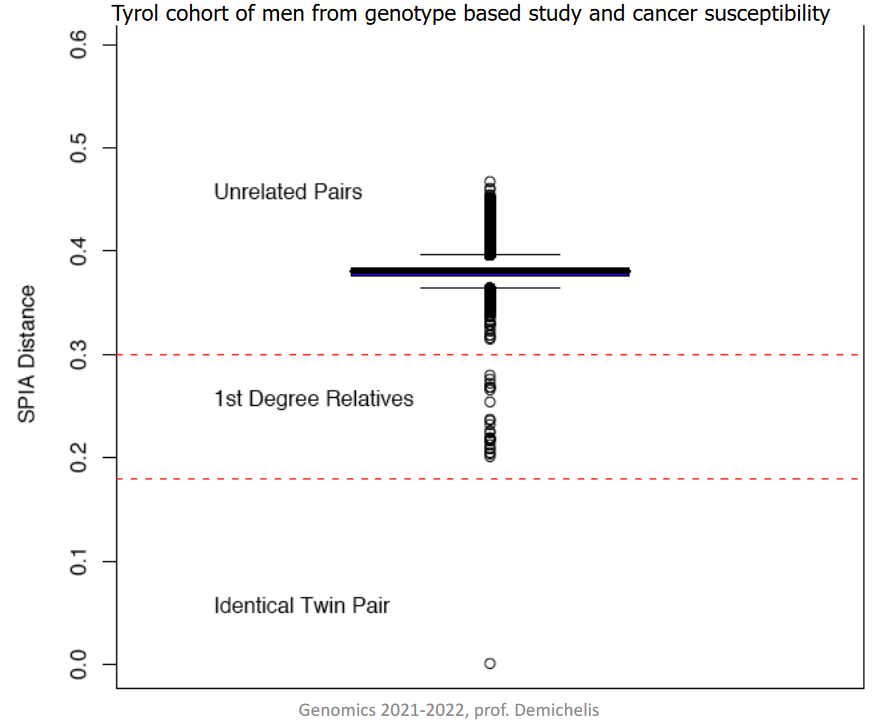
\includegraphics[width=0.60\textwidth]{IndividualsRelatedness.PNG}
  \label{fig: Relatedness of individuals}
\end{figure}

% #TODO have to clarify figure page 42

\subsection{Example 3: Cancer supscettibility test}
% #TODO to which data are you referring?
The data showed refers to a study were they were looking for polimorphisms that
increase the \textbf{likelihood of prostate cancer}. In these studies, if
relatives are present in the cohort, only one of them is taken to avoid skewing
the results. When looking for signs of cancer susceptibility by performing
genetic fingerprinting, the division based on the degree of relativeness was
determined 'for free' and could be used to remove unwanted samples from the
cohort.


\subsection{Genetic structure of the human population}

Undestanding the genetic structure of human populations is of fundamental
interest to medial, forensic and anthropological sceinces. 

The goal of association studies is to \underline{\textbf{identify DNA variants}
that affect disease risk} or other \underline{traits of interest}. However,
association studies can be confounded by differences in ancestry. \\
	
\textbf{Misleading results} could arise if individuals selected as disease cases
have different ancestry, on average, than healthy controls. The differences in
the markers wouldn't be due to the disease itself at this point, instead it
would be caused by the different origin. If in a study all controls are of the
same ethnicity and the test is done on an individual of a different ethnicity
than the test is biased. If we run a GWAS study using two ethnicities and we
want to uset the same markers of susceptibility worldwide, it won't work. \\

Especially in medicine and in the study of human evolution it is important to
\textbf{track the genetic background of individuals} that are involved in
studies in order to understand if the individuals are form a homogeneous
population or from genetically distant ones. More and more, clinical studies
must have declarations of the checks and interpretation of the data of the
genetic background of the individuals present in the study. It is very important
to come to results for which we know exactly what is the applicability. To avoid
spurious results, \underline{association studies often restrict their focus to a
single continental group}.\\

Advances in high-throughput genotyping technology have improved the
understanding of global patterns of human genetic variation and suggest the
potential to use large sample sets to \textbf{uncover variation among closely
spaced populations}. One important piece of information to consider when
developing methods to understand the genetic structure of a population, is to
think in term of variance, which is also relevant for human diseases. Many SNPs
have different \underline{MAFs} in different populations. If we use those, and
are able to have all of them in a simple computational way, we could be able to
infer what is one individual's genetic background in terms of origins (e.g.
chinese origins).\\

The easiest mathematical approach to assess how well SNPs can distinguish
ethnicity is by using \textbf{Principal Component Analysis (PCA)}. By running a
very simple PCA on a set of SNPs including SNPs with different MAF in different
populations we can, in a space, distinguish different ethnical groups. And we
could also start thinking at individuals' origins.\\

\emph{How accuratley can one predict an individuals geographic-ethnical
background based upon his/her geentic barcode?}

% study seen in the slides
\subsubsection{Example paper: 'Genes mirror geography within Europe'}

In the \href{https://www.ncbi.nlm.nih.gov/pmc/articles/PMC2735096/}{study seen
during lectures} they used a 500.000 (500k) single nucleotide polymorphism
array. Information about the country of origin of grandparents, parents and
other relatives was used to determine the geographical location that best
represents each individual ancestry. They run a combined study where they used a
supervised search to find the best SNPs to make inference and then they tested
it on another set of individuals. By using high confidence data (individuals
with high confidence origin data) and by using the genotypes of highly
informative SNPs for specific region-related inheritance, they were able to
\textbf{rebuild the map of some of the countries in Europe}
\ref{fig:PCA_countries}. \\

% immagine paper 
\begin{figure}[ht]
	\centering
	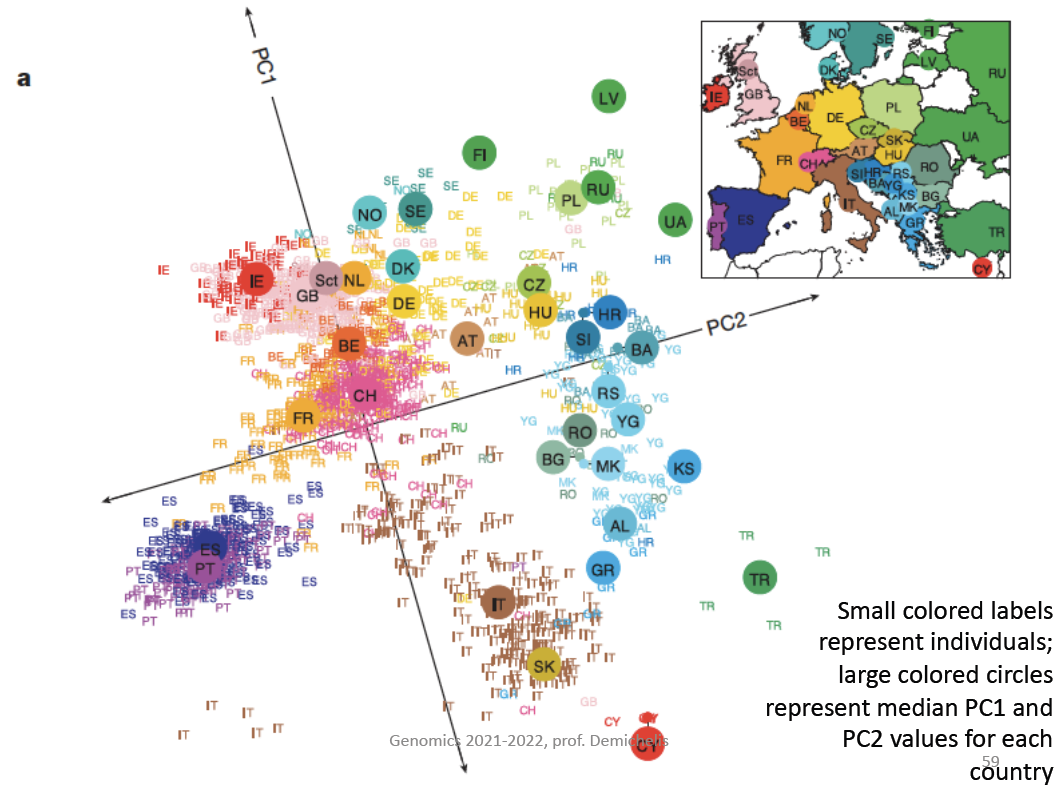
\includegraphics[width=1\textwidth]{PCA.PNG}
	\caption{Distinction of European regions thanks to SNPs.}
	\label{fig:PCA_countries}
\end{figure}

It is true that by using properly selected variants it is possible to
distinguish \textbf{individuals coming from different countries}. The way those
SNPs are selected is very similar to the process saw for genetic fingerprint,
but pushing for the selection of variants that are different in terms of MAF in
different populations. 

Clusters that are a bit more dense and distant from the others (like the
Spain/Portugal cluster) could be due to the fact that many SNPs selected are
typical of that area and are therefore able to maximize the difference between
that area and the others (so it is a data-related 'issue').
% 
% immagine 
\begin{figure}[ht]
	\centering
	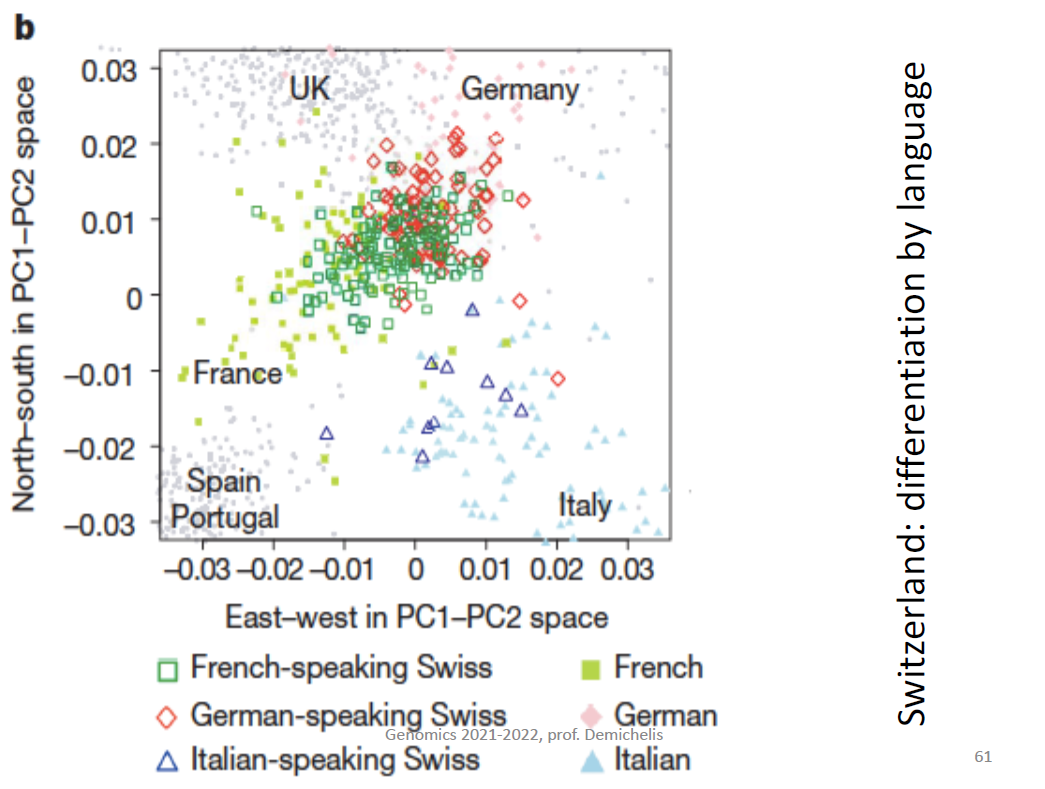
\includegraphics[width=0.8\textwidth]{PCA_swiss.PNG}
	\caption{\label{fig: PCA_swiss}}
\end{figure}

Focusing on Switzerland, they could even make inference on the linguistic canton
\ref{fig: PCA_swiss}. It is possibly true that in country where some regions
have very different cultures (e.g. marriage within the same area) might be
different between each other. 


\subsubsection{Summary and notes}
\textbf{Low-frequency alleles} tend to be the result of a recent mutation and
are expected to geographically cluster around the location at which the mutation
first arose. Hence, they can be highly informative about the \textbf{fine-scale}
population structure.

Despite low average levels of genetic differentiation among Europeans, close
correspondence between genetic and geographic distances was found. When mapping
the genetic basis of a disease phenotype, spurious associations can arise if
genetic structure is not properly accounted for.



\subsection{SPIA Assay} \label{subsect: SPIA} In a hand on lesson we performed
ourselves a SNP-based genetic distance test using the R package 'SPIAssay'. You
can find an R Markdown of that lesson in the folder 'Additional material'. 